%&../settings/preamble.main

\ifsubfile
\pagestyle{plain}
\setcounter{chapter}{5}

% arara: pdflatex: { options: ["--output-directory=../build"], draft: yes, synctex: no }
% arara: pdflatex: { options: ["--output-directory=../build"], synctex: no }
\begin{document}
\fi
\chapter{Alberi Binari di Ricerca}

\section{Introduzione}

Facciamo un breve ripasso della struttura dati dizionario.
La struttura dati dizionario è un insieme dinamico che implementa le seguenti funzionalità:
\begin{itemize}
	\item \Item \dictLookup{\Item \(v\)} permette di cercare per una certa chiave;
	\item \dictInsert{\Item \(k\), \Item \(v\)} permette di associare una chiave ad un valore;
	\item \dictRemove{\Item \(k\)} permette di rimuovere una certa associazione chiave-valore.
\end{itemize}

\begin{table}[H]
	\centering
	% \captionsetup{format=hang}
	\caption{Possibili implementazioni della struttura dati dizionario\\e relative complessità}
	\label{tab:complessita-implementazioni-dizionario}
	\begin{tabular}{@{} l *{3}{c} @{}}
	\toprule
		Struttura dati & \dictLookup & \dictInsert & \dictRemove\\
	\midrule
	Vettore ordinato & \(\Omicron(\log n)\) & \(\Omicron(n)\) & \(\Omicron(n)\)\\
	Vettore non ordinato & \(\Omicron(n)\) & \({\Omicron(1)}^{*}\) & \({\Omicron(1)}^{*}\)\\
	Lista non ordinata & \(\Omicron(n)\) & \({\Omicron(1)}^{*}\) & \({\Omicron(1)}^{*}\)\\
	\bottomrule
	\end{tabular}

	\smallskip
	{\small	* assumendo che l'elemento sia già stato trovato, \(\Omicron(n)\) altrimenti.}
\end{table}

Ora vedremo la struttura dati dizionario implementata come un albero binario di ricerca.

L'idea che ha portato allo sviluppo degli alberi binari di ricerca è stata quella di portare la ricerca binaria (o dicotomica) negli alberi, avendo quindi un meccanismo dinamico per la memorizzazione delle informazioni ma basandosi sul meccanismo della ricerca binaria per recuperarle.

Le associazioni chiave-valore vengono memorizzate in un albero binario.
Ogni nodo contiene una coppia (\(u\).\varKey, \(u\).\varValue).
Le chiavi devono appartenere ad un insieme \emph{totalmente ordinato}, ossia dev'essere possibile stabilire, date due chiavi, una relazione di precendenza fra di loro.

\begin{property*}
Le seguenti proprietà permettono di realizzare un algoritmo di ricerca dicotomica:
\begin{enumerate}
	\item Le chiavi contenute nei nodi del sottoalbero sinistro di \(u\) sono minori di \(u\).\varKey;
	\item Le chiavi contenute nei nodi del sottoalbero destro di \(u\) sono maggiori di \(u\).\varKey.
\end{enumerate}
\end{property*}

\begin{note}
Queste proprietà valgono per ogni nodo e riguardano l'intero sottoalbero.
\end{note}

Vedremo un algoritmo per verificare se un albero binario è un albero binario di ricerca più avanti (\verifyABR), il quale controllerà se queste proprietà sono soddisfatte.

\clearpage
\begin{algorithm}[H]
	\caption{Specifica Alberi Binari di Ricerca (\textsc{ABR})}
	%&../preamble

% arara: pdflatex: { synctex: no }
% arara: latexmk: { clean: partial }
\ifstandalone
\begin{document}
\begin{algorithm}[H]
\fi

\begin{minipage}[t]{.45\textwidth}
\BlankLine
\tcp{CONTENUTO DI UN NODO}

\BlankLine
\Tree \varParent\;
\Tree \varLeft\;
\Tree \varRight\;
\Item \varKey\;
\Item \varValue\;

\BlankLine
\tcp{GETTERS}

\BlankLine
\Tree \treeParent\;
\Tree \treeLeft\;
\Tree \treeRight\;
\Item \treeKey\;
\Item \treeValue\;

% \columnbreak
% \vspace{15pt}
% \vphantom{0pt}
\end{minipage}\hfill%
\begin{minipage}[t]{.45\textwidth}

\BlankLine
\tcp{ORDINAMENTO}

\BlankLine
\Tree \succNode{\Tree \(t\)}\;
\Tree \predNode{\Tree \(t\)}\;
\Tree \minNode\;
\Tree \maxNode\;

\BlankLine
\tcp{FUNZIONI DIZIONARIO}

\BlankLine
\Item \dictLookup{\Item \(k\)}\;
\dictInsert{\Item \(k\), \Item \(v\)}\;
\dictRemove{\Item \(k\)}\;

\BlankLine
\tcp{FUNZIONI INTERNE}

\BlankLine
\Item \lookupNode\;
\insertNode{\Tree \(T\), \Item \(k\), \Item \(v\)}\;
\removeNode{\Tree \(T\), \Item \(k\)}\;
\end{minipage}
\BlankLine

\ifstandalone
\end{algorithm}
\end{document}
\fi

\end{algorithm}

\subsection*{Ricerca di un nodo}

\begin{algorithm}[H]
	\caption{Ricerca di un nodo in un dizionario realizzato tramite \textsc{ABR}}
	%&../preamble

% arara: pdflatex: { synctex: no }
% arara: latexmk: { clean: partial }
\ifstandalone
\begin{document}
\begin{algorithm}[H]
\fi

\BlankLine
\prototype{\Int \dictLookup{\Item \(k\)}}{
	\Tree \(t\) \Assign \lookupNode{\(tree, k\)}\;

	\BlankLine
	\eIf{\(t \Neq \Nil\)}{
		\Return \(t\).\treeValue\;
	}{
		\Return \Nil\;
	}
}

\BlankLine
% \tcp{Restituisce il nodo dell'albero \(t\)}
% \tcp{che contiene la chiave \(k\),}
% \tcp{se presente, \Nil altrimenti}
\tcp{RICERCA DI UN NODO, iterativa}
\prototype{\Tree \lookupNode{\Tree \(T\), \Item \(k\)}}{
	\Tree \(u \Assign T\) \Comment*[l]{parto dalla radice}

	\BlankLine
	\While{\(u \Neq \Nil\) \And \(u.\treeKey \Neq k\)}{
		\(u\) \Assign \iif{\(k < u.\treeKey, u.\treeLeft, u.\treeRight\)}\;
	}
}

\BlankLine
\tcp{RICERCA DI UN NODO, ricorsiva}
\prototype{\Tree \lookupNode{\Tree \(T\), \Item \(k\)}}{
	\eIf{\(T \Equal \Nil\) \Or \(T.\treeKey \Equal k\)}{
		\Return \(T\)\;
	}{
		\Return \lookupNode{\iif{\(k < u.\treeKey, u.\treeLeft, u.\treeRight\)}, \(k\)}\;
	}
}
\BlankLine

\ifstandalone
\end{algorithm}
\end{document}
\fi

\end{algorithm}

\clearpage
\subsection*{Ricerca del minimo e del massimo}

\begin{algorithm}[H]
	\caption{Ricerca del minimo e del massimo in un dizionario realizzato tramite \textsc{ABR}}
	%&../preamble

% arara: pdflatex: { synctex: no }
% arara: latexmk: { clean: partial }
\ifstandalone
\begin{document}
\begin{algorithm}[H]
\fi

\begin{minipage}{.5\textwidth}
\BlankLine
\tcp{RICERCA DEL MINIMO}
\prototype{\Tree \minNode{\Tree \(T\)}}{
	\Tree \(u = T\) \Comment*[l]{parto dalla radice}

	\BlankLine
	\While{\(u.\treeLeft \Neq \Nil\)}{
		\(u \Assign u.\treeLeft\)\;
	}

	\BlankLine
	\Return \(u\)\;
}

% \vspace{-5pt}
% \vphantom{0pt}
\end{minipage}%
\begin{minipage}{.5\textwidth}

\BlankLine
\tcp{RICERCA DEL MASSIMO}
\prototype{\Tree \maxNode{\Tree \(T\)}}{
	\Tree \(u = T\) \Comment*[l]{parto dalla radice}

	\BlankLine
	\While{\(u.\treeRight \Neq \Nil\)}{
		\(u \Assign u.\treeRight\)\;
	}

	\BlankLine
	\Return \(u\)\;
}
\end{minipage}
\BlankLine

\ifstandalone
\end{algorithm}
\end{document}
\fi

\end{algorithm}

\subsection*{Ricerca del predecessore, successore}

\begin{algorithm}[H]
	\caption{Ricerca del predecessore e del successore di un nodo in un dizionario realizzato tramite \textsc{ABR}}
	%&../preamble

% arara: pdflatex: { synctex: no }
% arara: latexmk: { clean: partial }
\ifstandalone
\begin{document}
\begin{algorithm}[H]
\fi

\begin{minipage}{.5\textwidth}
\BlankLine
\tcp{RICERCA DEL PREDECESSORE}
\prototype{\Tree \predNode{\Tree \(t\)}}{

	\BlankLine
	\If{\(t \Equal \Nil\)}{
		\Return \(t\)\;
	}

	\BlankLine
	\eIf{\(t.\alert{\treeLeft} \Neq \Nil\)}{
	\lnlset{sx-does-exists}{1}%
		\Return \(\alert{\maxNode{t.\treeLeft}}\)\;
	}{\lnlset{sx-not-exists}{2}%
		\Tree \(p \Assign t.\treeParent\)\;

		\BlankLine
		\While{\(p \Neq \Nil\) \And \(t \Equal p.\alert{\treeLeft}\)}{
			\(t \Assign p\) \Comment*[l]{padre}
			\(p \Assign p.\treeParent\) \Comment*[l]{nonno}
		}
	}

	\BlankLine
	\Return \(p\)\;
}

% \vspace{-5pt}
% \vphantom{0pt}
\end{minipage}%
\begin{minipage}{.5\textwidth}

\BlankLine
\tcp{RICERCA DEL SUCCESSORE}
\prototype{\Tree \succNode{\Tree \(t\)}}{

	\BlankLine
	\If{\(t \Equal \Nil\)}{
		\Return \(t\)\;
	}

	\BlankLine
	\eIf{\(t.\alert{\treeRight} \Neq \Nil\)}{
	\lnlset{dx-dies-exists}{3}%
		\Return \(\alert{\minNode{t.\alert{\treeRight}}}\)\;
	}{\lnlset{dx-not-exists}{4}%
		\Tree \(p \Assign t.\treeParent\)\;

		\BlankLine
		\While{\(p \Neq \Nil\) \And \(t \Equal p.\alert{\treeRight}\)}{
			\(t \Assign p\)\;
			\(p \Assign p.\treeParent\)\;
		}
	}

	\BlankLine
	\Return \(p\)\;
}
\end{minipage}
\BlankLine

\ifstandalone
\end{algorithm}
\end{document}
\fi

\end{algorithm}

\begin{enumerate}[label={\footnotesize\ttfamily (\arabic*)}]
	\item \(u\) ha figlio sinistro: il predecessore è il massimo del sottoalbero sinistro di \(u\);
	\item \(u\) non ha figlio sinistro: risalendo attraverso i padri, il predecessore è il primo avo \(v\) tale per cui \(u\) sta nel sottoalbero destro di \(v\);
	\item \(u\) ha figlio destro: il successore è il minimo del sottoalbero destro di \(u\);
	\item \(u\) non ha figlio destro: risalendo attraverso i padri, il sucessore è il primo avo \(v\) tale per cui \(u\) sta nel sottoalbero sinistro di \(v\).
\end{enumerate}

\begin{note}
Posso trovare \Nil se passo alla funzione \succNode il nodo massimo o alla funzione \predNode il minimo (usciranno dal ciclo restituendo \(p\) che sarà pari a \Nil).
\end{note}

\clearpage
\subsection*{Inserimento di un nodo}

La funzione \insertNode inserisce un'associazione chiave-valore \((k,v)\) nell'albero \(T\).
Se la chiave è già presente, sostituisce il valore associato;
altrimenti, viene inserita una nuova associazione.
Se l'albero è vuoto (\(T \Equal \Nil\)) restituisce il primo nodo dell'albero, altrimenti restituisce la radice di \(T\) inalterata.

La funzione ausiliaria \shortcut si occupa di inserire il nodo collegandolo al corretto genitore.

\begin{algorithm}[H]
	\caption{Inserimento di un nodo in un \textsc{Dictionary} realizzato tramite \textsc{ABR}}
	%&../preamble

% arara: pdflatex: { synctex: no }
% arara: latexmk: { clean: partial }
\ifstandalone
\begin{document}
\begin{algorithm}[H]
\fi

\BlankLine
\tcp{IMPLEMENTAZIONE DIZIONARIO}
\prototype{\dictInsert{\Item \(k\), \Item \(v\)}}{
	\(tree\) \Assign \insertNode{\(tree, k, v\)}\;
}

\ifstandalone
\end{algorithm}
\end{document}
\fi

	%&../preamble

% arara: pdflatex: { synctex: no }
% arara: latexmk: { clean: partial }
\ifstandalone
\begin{document}
\begin{algorithm}[H]
\fi

\BlankLine
\tcp{INSERIMENTO DI UN NODO}
\prototype{\Tree \insertNode{\Tree \(T\), \Item \(k\), \Item \(v\)}}{
	\Tree \(p \Assign \Nil\) \Comment*[l]{padre}
	\Tree \(u \Assign T\) \Comment*[l]{parto dalla radice}

	\BlankLine
	\tcp{cerco posizione inserimento}
	\While{\(u \Neq \Nil\) \And \(u.\treeKey \Neq k\)}{
		\(p \Assign u\)\;
		\(u\) \Assign \iif{\(k < u.\treeKey, u.\treeLeft, u.\treeRight\)}\;
	}

	\BlankLine
	\eIf{\(u \Neq \Nil\) \And \(u.\treeKey \Equal k\)}{
		\tcp{la chiave è già presente, aggiorno il valore}

		\BlankLine
		\(u.\treeValue \Assign v\)\;
	}{
		\tcp{la chiave non è presente}
		\tcp{creo un nodo coppia chiave-valore}
		\Tree \(new\) \Assign \treeConstructor{\(k, v\)}\;

		\BlankLine
		\tcp{collego il nodo creato}
		\shortcut{\(p, new, k\)}\;

		\BlankLine
		\If{\(p \Equal \Nil\)}{
			\(T \Assign new\) \Comment*[l]{primo nodo ad essere inserito}
		}
	}

	\BlankLine
	\tcp{restituisco l'albero non modificato o il nuovo nodo}
	\Return \(T\)\;
}

\ifstandalone
\end{algorithm}
\end{document}
\fi

	%&../preamble

% arara: pdflatex: { synctex: no }
% arara: latexmk: { clean: partial }
\ifstandalone
\begin{document}
\begin{algorithm}[H]
\fi

\BlankLine
\tcp{collega un nodo padre \(p\) ad un nodo figlio \(u\)}
\prototype{\shortcut{\Tree p, \Tree u, \Item x}}{
	\If{\(u \Neq \Nil\)}{
		\tcp{il nodo è stato cancellato}
		\(u\).\treeParent \Assign \(p\) \Comment*[l]{registro il padre}
	}

	\BlankLine
	\If{\(p \Neq \Nil\)}{
		\tcp{collego il nodo sul figlio corretto}
		\(u\) \Assign \iif{\(x < p.\treeKey, p.\treeLeft, p.\treeRight\)}\;
	}
}

\ifstandalone
\end{algorithm}
\end{document}
\fi

\end{algorithm}

\clearpage
\subsection*{Rimozione di un nodo}

Rimuove il nodo contenente la chiave \(k\) dall'albero \(T\), restituisce la radice dell'albero (potenzialmente cambiata).

% TODO assicurarsi che questo algoritmo sia in una pagina pari, in modo tale da avere la spiegazione grafica sulla destra
\begin{algorithm}[H]
	\caption{Rimozione di un nodo in un \textsc{Dictionary} realizzato tramite \textsc{ABR}}
	%&../preamble

% arara: pdflatex: { synctex: no }
% arara: latexmk: { clean: partial }
\ifstandalone
\begin{document}
\begin{algorithm}[H]
\fi

\BlankLine
\tcp{IMPLEMENTAZIONE DIZIONARIO}
\prototype{\dictRemove{\Item \(k\)}}{
	\Tree \(tree \Assign \removeNode{tree, k}\)\;
}

\ifstandalone
\end{algorithm}
\end{document}
\fi

	%&../preamble

% arara: pdflatex: { synctex: no }
% arara: latexmk: { clean: partial }
\ifstandalone
\begin{document}
\begin{algorithm}[H]
\fi

\BlankLine
\tcp{RIMOZIONE DI UN NODO}
\prototype{\Tree \removeNode{\Tree \(T\), \Item \(k\)}}{
	% NOTE viene dichiarato ma non viene utilizzato
	% \Tree \(t\)\;

	\BlankLine
	\tcp{individuo il nodo da rimuovere}
	\Tree \(u \Assign\) \lookupNode{\(T, k\)}\;

	\BlankLine
	\tcp{se il nodo da rimuovere è presente nell'albero\dots}
	\If{\(u \neq \Nil\)}{
		\lnl{case:primo-caso}%
		\tcp{\dots e non ha figli}
		\uIf{\(u.\treeLeft \Equal \Nil\) \And \(u.\treeRight \Equal \Nil\)}{
		% \uIf(\tcp*[h]{nessun figlio}){\(u.\treeLeft \Equal \Nil\) \And \(u.\treeRight \Equal \Nil\)}{
			\If(\tcp*[h]{se esiste il padre}){\(u.\treeParent \Neq \Nil\)}{
				\shortcut{\(u.\treeParent, \Nil, k\)} \Comment*[l]{rimuovo il puntatore al figlio}
			}

			\BlankLine
			\tcp{rimuovo direttamente il nodo}
			\delete \(u\)\;
		}\lnlset{terzo-caso}{3}%
		\tcp{\dots ed ha due figli}
		\uIf{\(u.\treeLeft \neq \Nil\) \And \(u.\treeRight \neq \Nil\)}{
		% \uIf(\tcp*[h]{due figli}){\(u.\treeLeft \neq \Nil\) \And \(u.\treeRight \neq \Nil\)}{

			\BlankLine
			\Tree \(s\) \Assign \succNode \Comment*[l]{individuo il successore}

			\BlankLine
			\shortcut{\(s.\treeParent, s.\treeRight, s.\treeKey\)} \Comment*[l]{collego il sottoalbero destro}

			\BlankLine
			\tcp{copio il successore}
			\tcp{nella posizione del nodo rimosso}
			\(u.\treeKey \Assign s.\treeKey\)\;
			\(u.\treeValue \Assign s.\treeValue\)\;

			\BlankLine
			\tcp{rimuovo il successore}
			\delete \(s\)\;
		}\lnl{case:secondo-caso}%
		\tcp{\dots ed ha un solo figlio (sinistro)}
		\uIf{\(u.\treeLeft \neq \Nil\) \And \(u.\treeRight \Equal \Nil\)}{
		% \uIf(\tcp*[h]{solo un figlio (sinistro)}){\(u.\treeLeft \neq \Nil\) \And \(u.\treeRight \Equal \Nil\)}{

			\BlankLine
			\shortcut{\(u.\treeParent, u.\treeLeft, k\)} \Comment*[l]{collega il figlio al padre}

			\BlankLine
			\If(\tcp*[h]{se il padre non esiste}){\(u.\treeParent \Equal \Nil\)}{
				\(T \Equal u.\treeRight\) \Comment*[l]{il figlio diventa la radice}
			}
		}
		\tcp{\dots ed ha un solo figlio (sinistro)}
		\Else{
		% \Altrimenti(\tcp*[h]{solo un figlio (destro)}){

			\BlankLine
			\shortcut{\(u.\treeParent, u.\treeRight, k\)} \Comment*[l]{collega il figlio al padre}

			\BlankLine
			\If(\tcp*[h]{se il padre non esiste}){\(u.\treeParent \Equal \Nil\)}{
				\(T \Equal u.\treeRight\) \Comment*[l]{il figlio diventa la radice}
			}
		}
	}

	\BlankLine
	\tcp{restituisco la radice}
	\Return \(T\)\;
}

\ifstandalone
\end{algorithm}
\end{document}
\fi

	% %&../preamble

% arara: pdflatex: { synctex: no }
% arara: latexmk: { clean: partial }
\ifstandalone
\begin{document}
\begin{algorithm}[H]
\fi

\BlankLine
\tcp{collega un nodo padre \(p\) ad un nodo figlio \(u\)}
\prototype{\shortcut{\Tree p, \Tree u, \Item x}}{
	\If{\(u \Neq \Nil\)}{
		\tcp{il nodo è stato cancellato}
		\(u\).\treeParent \Assign \(p\) \Comment*[l]{registro il padre}
	}

	\BlankLine
	\If{\(p \Neq \Nil\)}{
		\tcp{collego il nodo sul figlio corretto}
		\(u\) \Assign \iif{\(x < p.\treeKey, p.\treeLeft, p.\treeRight\)}\;
	}
}

\ifstandalone
\end{algorithm}
\end{document}
\fi

\end{algorithm}

\clearpage
\begin{enumerate}[label={\footnotesize\ttfamily (\arabic*)}]
	\item se il nodo da eliminare \(u\) non ha figli: lo si elimina semplicemente, in quanto togliere una foglia non altera le proprietà di ordinamento dell'albero;
	% NOTE aggiustamenti per fare rientrare tutto in una pagina
	\vspace{-5pt}
	\begin{figure}[H]\centering
		\hfill
		\begin{subfigure}[t]{.3\linewidth}
			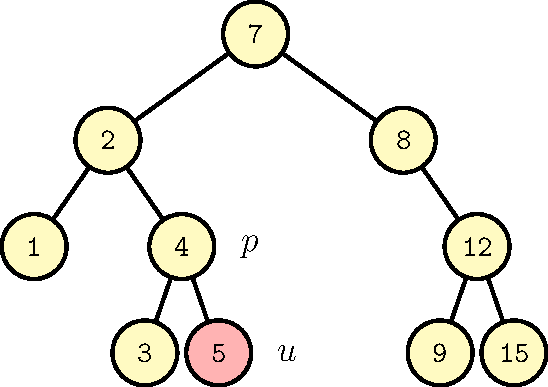
\includegraphics[width=\linewidth, page=1]{tree-abr-delete1}
			\caption{Individuazione nodo foglia}
		\end{subfigure}
		\hfill
		\begin{subfigure}[t]{.3\linewidth}
			\includegraphics[width=\linewidth, page=2]{tree-abr-delete1}
			\caption{Rimozione del nodo foglia}
		\end{subfigure}
		\hfill\null
	\end{figure}
	% NOTE aggiustamenti per fare rientrare tutto in una pagina
	\vspace{-15pt}
	\item se il nodo da eliminare ha un solo figlio \(f\) (destro o sinistro): si elimina \(u\) e si collega \(f\) all'ex-padre \(p\) di \(u\) in sostituzione di \(u\) (tramite la funzione \shortcut);
	le proprietà di ordinamento non vengono alterate in quanto tutti i nodi del sottoalbero destro di \(p\) sono maggiori di \(p\) stesso;
	% NOTE aggiustamenti per fare rientrare tutto in una pagina
	\vspace{-5pt}
	\begin{figure}[H]
		\begin{subfigure}[t]{.3\linewidth}
			\includegraphics[width=\linewidth, page=3]{tree-abr-delete1}
			\caption{Individuazione nodo \(u\) da eliminare}
		\end{subfigure}
		\hfill
		\begin{subfigure}[t]{.3\linewidth}
			\includegraphics[width=\linewidth, page=4]{tree-abr-delete1}
			\caption{Rimozione nodo \(u\)}
		\end{subfigure}
		\hfill
		\begin{subfigure}[t]{.3\linewidth}
			\includegraphics[width=\linewidth, page=5]{tree-abr-delete1}
			\caption{Collegamento del sottoalbero \(f\) di \(u\) al padre \(p\) di \(u\)}
		\end{subfigure}
	\end{figure}
	% NOTE aggiustamenti per fare rientrare tutto in una pagina
	\vspace{-15pt}
	\item se il nodo da eliminare \(u\) ha due figli: cerchiamo di ricadere nel caso {\footnotesize\ttfamily (2)};
	\begin{enumerate*}
		\item individuiamo il successore (predecessore) \(s\) di \(u\), il quale è il più piccolo valore maggiore di \(u\) (il più grande valore minore di \(u\)) e di conseguenza non ha figli sinistri (non ha figli destri);
		\item si \enquote{stacca} il successore \(s\);
		\item si collega l'eventuale figlio destro di \(s\) al padre (tramite la funzione \shortcut) in quanto trovandosi nel sottoalbero sinistro del nonno vuol dire che sicuramente il suo valore non è maggiore del padre di \(s\);
		\item si copia \(s\) su \(u\), si rimuove il nodo \(s\), così facendo rispetto comunque l'ordine parziale.
	\end{enumerate*}
	% NOTE aggiustamenti per fare rientrare tutto in una pagina
	\vspace{-5pt}
	\begin{figure}[H]
		\hfill
		\begin{subfigure}[t]{.45\linewidth}
			\includegraphics[width=\linewidth, page=2]{tree-abr-delete2}
			\caption{Individuiamo il successore \(s\) di \(u\)}
		\end{subfigure}
		\hfill
		\begin{subfigure}[t]{.45\linewidth}
			\includegraphics[width=\linewidth, page=3]{tree-abr-delete2}
			\caption{Si \enquote{stacca} il successore \(s\)}
		\end{subfigure}
		\hfill\null

		\vspace{10pt}

		\hfill
		\begin{subfigure}[t]{.45\linewidth}
			\includegraphics[width=\linewidth, page=4]{tree-abr-delete2}
			\caption{Si collega l'eventuale figlio destro di \(s\) al padre}
		\end{subfigure}
		\hfill
		\begin{subfigure}[t]{.45\linewidth}
			\includegraphics[width=\linewidth, page=5]{tree-abr-delete2}
			\caption{Si copia \(s\) su \(u\), si rimuove il nodo \(s\)}
		\end{subfigure}
		\hfill\null

		% NOTE rimosso perché la spiegazione risulta ugualmente chiara, e non ci starebbe tutto in una pagina diciamocelo
		% \vspace{10pt}
		%
		% \hfill
		% \begin{subfigure}[t]{.45\linewidth}
		% 	\includegraphics[width=\linewidth, page=5]{tree-abr-delete2}
		% 	\caption{bla bla bla}
		% \end{subfigure}
		% \hfill\null
	\end{figure}
\end{enumerate}

\clearpage
\subsection*{Costo computazionale delle operazioni}

Tutte le operazioni sono confinate ai nodi posizionati lungo un cammino semplice dalla radice ad una foglia.
Quindi se l'altezza dell'albero è definita come \(h\), il tempo di ricerca ha complessità \(\Omicron(h)\).

Il caso pessimo è rappresentanto da un albero sbilanciato completamente a destra o completamente a sinistra.
Questo caso può accadere quando si inseriscono ordinatamente i dati nell'albero.
Questo caso, dove l'altezza \(h = n\) porta ad una complessità \(\Omicron(n)\).

Mentre il caso ottimo è rappresentanto da un albero perfettamente bilanciato.
Nell'esempio è mostrato un albero perfetto con \(2^h - 1\) nodi, dove \(h\) è l'altezza.
In questo caso la complessità è pari a \(\Omicron(\log n)\), ad esempio con \(h = 2^3 - 1\) la complessità è \(\Omicron(\log h) = \Omicron(\log 7) < 3\).

Ci domandiamo quindi quale sia l'altezza media di un albero binario di ricerca.
Il caso \enquote{semplice} è quello di considerare che gli inserimenti avvengano in maniera statisticamente uniforme, è possibile dimostrare che l'altezza media è \(\Omicron(\log n)\), mentre il caso generale, ossia quello in cui avvengono sia inserimenti che cancellazioni è di difficile trattazione. Per evitare questa casistica si utilizzano varie tecniche per mantenere l'albero bilanciato.
Per capire queste tecniche abbiamo prima bisogno di fissare un concetto.
\begin{definition}[Fattore di bilanciamento]
Il fattore di bilanciamento \(\beta(v)\) di un nodo \(v\) è la massima differenza di altezza fra i sottoalberi di \(v\).
\end{definition}

Negli anni sono state usate diverse tecniche, ora in disuso:
\begin{itemize}
	\item Alberi AVL (1962): \(\beta(v) \leqslant 1\) per ogni nodo \(v\), il bilanciamento dell'albero avveniva tramite rotazioni;
	\item B-Alberi (1972): \(\beta(v) = 0\) per ogni nodo \(v\), sono specializzati per strutture in memoria secondaria;
	\item Alberi 2-3 (1983): \(\beta(v) = 0\) per ogni nodo \(v\), in cui ogni nodo può avere o 2 o 3 figli, se ad un nodo viene aggiunto un ulteriore figlio, il ramo viene spezzato in due rami con 2 figli ciascuno, mentre se ad un ramo con 2 figli ne viene tolto uno allora l'unico figlio rimanente viene collegato al padre, questo potrebbe riportare il problema al primo caso; il bilanciamento viene ottenuto quindi tramite merge/split, il grado è variabile.
\end{itemize}

\begin{note}[Meccanismo di rotazione]
Il meccanismo di rotazione ci permette di abbassare il fattore di sbilanciamento rispettando le proprietà di ordinamento parziale.
\end{note}

\clearpage
\section{Alberi Binari di Ricerca bilanciati}

\begin{definition}[Albero Red-Black]
Un albero red-black è un albero binario di ricerca in cui:
\begin{itemize}
	\item ogni nodo è colorato di rosso o di nero;
	\item le chiavi vengono mantenute solo nei nodi interni dell'albero;
	\item le foglie sono costituite solo da nodi speciali \textbf{Nil}.
\end{itemize}
\end{definition}

I nodi speciali \textbf{Nil} sono dei nodi sentinella il cui unico scopo è quello di evitare di trattare diversamente i puntatori ai nodi, dai puntatori \Nil;
infatti al posto di un puntatore \Nil si usa un puntatore ad un nodo \textbf{Nil};
in memoria ne esiste solo uno per motivi di economia.
I nodi con figli \textbf{Nil} sono le foglie nell'albero binario di ricerca corrispondente.

Un albero red-black deve rispettare i seguenti vincoli:
\begin{enumerate}
	\item la radice è nera;
	\item tutte le foglie sono nere;
	\item entrambi i figli di un nodo rosso sono neri;
	\item ogni cammino semplice da un nodo \(u\) ad una delle foglie contenute nel sottoalbero radicato in \(u\) ha lo stesso numero di nodi neri.
\end{enumerate}

\begin{algorithm}[H]
	\caption{Specifica \textsc{Red-Black Tree}}
	%&../preamble

% arara: pdflatex: { synctex: no }
% arara: latexmk: { clean: partial }
\ifstandalone
\begin{document}
\begin{algorithm}[H]
\fi

\BlankLine
\tcp{CONTENUTO DI UN NODO}

\BlankLine
\Tree \varParent\;
\Tree \varLeft\;
\Tree \varRight\;
\Int \alert{\varColor} \Comment*[l]{\RED o \BLACK}
\Item \varKey\;
\Item \varValue\;

\BlankLine
\tcp{GETTERS}

\BlankLine
\Tree \treeParent\;
\Tree \treeLeft\;
\Tree \treeRight\;
\Int \treeColor\;
\Item \treeKey\;
\Item \treeValue\;

\ifstandalone
\end{algorithm}
\end{document}
\fi

\end{algorithm}

\begin{property*}[Altezza nera di un nodo \(v\)]
L'altezza nera \(b(v)\) di un nodo \(v\) è il numero di nodi neri lungo ogni percorso da \(v\) (escluso) ad ogni foglia (inclusa) del suo sottoalbero.
\end{property*}

\begin{property*}[Altezza nera di un albero Red-Black]
L'altezza nera di un albero Red-Black è pari all'altezza nera della sua radice.
\end{property*}

Entrambe le proprietà sono ben definite perché tutti i percorsi hanno lo stesso numero di nodi neri (per via della regola no.\ 4).

\clearpage
\subsection*{Esempi}

Nelle suguenti figure i nodi neri sono segnati in bianco, mentre quelli rossi sono segnati.

\begin{figure}[H]\centering
	\renewcommand{\subfigurename}{Es.}
	\renewcommand\thesubfigure{\arabic{subfigure}}
	\captionsetup[subfigure]{labelformat=simple, labelsep=space}
	\begin{subfigure}[t]{.48\linewidth}\centering
		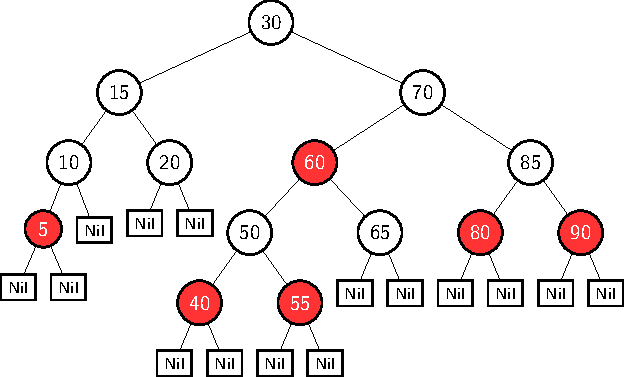
\includegraphics[width=\linewidth, page=1]{tree-rb-examples}
		\caption{Entrambi i figli di un nodo rosso sono neri (3),\\ma un nodo nero può avere figli neri.}
	\end{subfigure}
	\hfill
	\begin{subfigure}[t]{.48\linewidth}\centering
		\includegraphics[width=\linewidth, page=2]{tree-rb-examples}
		\caption{Ogni percorso da un nodo interno ad un nodo \textbf{Nil} ha lo stesso numero  di nodi neri (4).\\L'altezza nera di quest'albero è 3}
		\vspace{5pt}
	\end{subfigure}

	\begin{lemma}
	L'altezza totale di un albero è al più il doppio della sua altezza nera.
	\end{lemma}

	\begin{subfigure}[t]{.48\linewidth}\centering
		\includegraphics[width=\linewidth, page=2]{tree-rb-examples}
		\caption{Più colorazioni sono possibili (versione 1).\\L'altezza di questo albero è 3}
	\end{subfigure}
	\hfill
	\begin{subfigure}[t]{.48\linewidth}\centering
		\includegraphics[width=\linewidth, page=3]{tree-rb-examples}
		\caption{Più colorazioni sono possibili (versione 2).\\L'altezza di questo albero è 3}
	\end{subfigure}

	\begin{subfigure}[t]{.48\linewidth}\centering
		\includegraphics[width=\linewidth, page=4]{tree-rb-examples}
		\caption{Cambiare colorazione può cambiare l'altezza nera.\\L'altezza di questo albero è 3}
	\end{subfigure}
	\hfill
	\begin{subfigure}[t]{.48\linewidth}\centering
		\includegraphics[width=\linewidth, page=5]{tree-rb-examples}
		\caption{Cambiare colorazione può cambiare l'altezza nera.\\Stesso albero, l'altezza nera di questo albero è 2}
	\end{subfigure}
\end{figure}

% \clearpage
% \subsection*{Esercizio}
%
% \begin{figure}[ht]
% 	\caption*{Quasto albero può essere un albero Red-Black?}
% 	\vspace{5pt}
% 	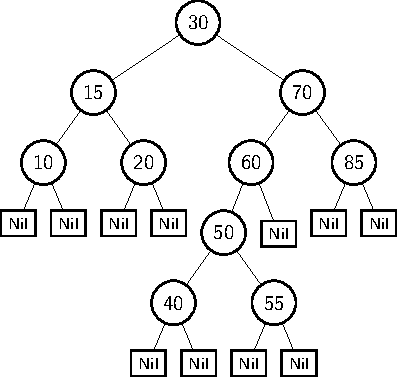
\includegraphics[width=\linewidth, height=4.5cm, keepaspectratio]{tree-rb-question}
% \end{figure}
% \vfill\null
% \clearpage

\clearpage
\subsection{Inserimento di un nodo}

Durante la modifica di un albero Red-Black è possibile che le condizioni di bilanciamento risultino violate.
Quando i vincoli Red-Black vengono violati si può agire in due modi:
\begin{itemize}
	\item modificando i colori nella zona della violazione;
	\item operando dei bilanciamenti dell'albero tramite rotazioni (a destra o a sinistra)
\end{itemize}

\subsection{Bilanciamento dell'albero}

\subsection*{Rotazione a sinistra}

\begin{algorithm}[H]
	% \caption{Rotazione di un \textsc{Red-Black Tree} a sinistra}
	\caption{Bilanciamento dell'albero tramite rotazione a sinistra}
	\setcounter{AlgoLine}{0}
	%&../preamble

% arara: pdflatex: { synctex: no }
% arara: latexmk: { clean: partial }
\ifstandalone
\begin{document}
\begin{algorithm}[H]
\fi

\BlankLine
\tcp{effettua una rotazione verso sinistra}
\prototype{\Tree \leftRotation{\Tree x}}{
	\lnl{case:primo-step}%
	\Tree \(y \Assign x.\treeRight\)\;
	\Tree \(p \Assign x.\treeParent\)\;

	\BlankLine
	\lnl{case:secondo-step}%
	\(x.\treeRight \Assign y.\treeLeft\) \Comment*[l]{il sottoalbero \(B\) diventa figlio destro di \(x\)}
	\If{\(y.\treeLeft \Neq \Nil\)}{
		\(y.\treeLeft.\treeParent \Assign x\)\;
	}

	\BlankLine
	\lnl{case:terzo-step}%
	\(y.\treeLeft \Assign x\) \Comment*[l]{\(x\) diventa figlio sinistro di \(y\)}
	\(x.\treeParent \Assign y\)\;

	\BlankLine
	\lnl{case:quarto-step}%
	\(y.\treeParent \Assign p\) \Comment*[l]{\(y\) diventa figlio di \(p\)}
	\If{\(p \Neq \Nil\)}{
		\eIf{\(p.\treeLeft \Equal x\)}{
			\(p.\treeLeft \Assign y\)
		}{
			\(p.\treeRight \Assign y\)
		}
	}

	\BlankLine
	\Return \(y\)\;
}

\ifstandalone
\end{algorithm}
\end{document}
\fi

\end{algorithm}

\begin{note}
Il disegno differisce minimamente da quello che si trova sulle slide per motivi di comodità nel disegnarli con \LaTeX{}
\end{note}
\begin{figure}[H]
	\renewcommand\thesubfigure{\arabic{subfigure}}
	\begin{subfigure}[t]{.23\linewidth}
		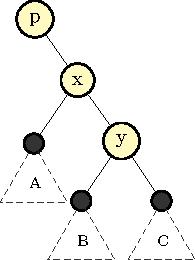
\includegraphics[width=\linewidth, page=1]{tree-rb-leftRotation}
		\caption{Stato iniziale}
	\end{subfigure}\hfill
	\begin{subfigure}[t]{.23\linewidth}
		\includegraphics[width=\linewidth, page=2]{tree-rb-leftRotation}
		\caption{Il sottoalbero \(B\) diventa figlio dx di \(x\)}
	\end{subfigure}\hfill
	\begin{subfigure}[t]{.23\linewidth}
		\includegraphics[width=\linewidth, page=3]{tree-rb-leftRotation}
		\caption{\(x\) diventa figlio sx di \(y\)}
	\end{subfigure}\hfill
	\begin{subfigure}[t]{.23\linewidth}
		\includegraphics[width=\linewidth, page=4]{tree-rb-leftRotation}
		\caption{\(y\) diventa figlio di \(p\),\\il vecchio padre di \(x\)}
	\end{subfigure}
	\caption{Esempio di rotazione a sinistra}
\end{figure}
\clearpage
\subsection*{Rotazione a destra}

La rotazione a destra è simmetrica e viene spiegata ed illustrata per completezza.

\begin{algorithm}[H]
	% \caption{Rotazione di un \textsc{Red-Black Tree} a destra}
	\caption{Bilanciamento dell'albero tramite rotazione a destra}
	\setcounter{AlgoLine}{0}
	%&../preamble

% arara: pdflatex: { synctex: no }
% arara: latexmk: { clean: partial }
\ifstandalone
\begin{document}
\begin{algorithm}[H]
\fi

\BlankLine
\tcp{effettua una rotazione verso destra}
\prototype{\Tree \rightRotation{\Tree x}}{
	\tcp{entrambi potrebbero essere \Nil}
	\lnl{case:primo-step}%
	\Tree \(y \Assign x.\treeLeft\)\;
	\Tree \(p \Assign x.\treeParent\)\;

	\BlankLine
	\lnl{case:secondo-step}%
	\(x.\treeLeft \Assign y.\treeRight\) \Comment*[l]{il sottoalbero \(B\) diventa figlio sinistro di \(x\)}
	\If{\(y.\treeRight \Neq \Nil\)}{
		\(y.\treeRight.\treeParent \Assign x\)\;
	}

	\BlankLine
	\lnl{case:terzo-step}%
	\(y.\treeRight \Assign x\) \Comment*[l]{\(x\) diventa figlio destro di \(y\)}
	\(x.\treeParent \Assign y\)\;

	\BlankLine
	\lnl{case:quarto-step}%
	\(y.\treeParent \Assign p\) \Comment*[l]{\(y\) diventa figlio di \(p\)}
	\If{\(p \Neq \Nil\)}{
		\If{\(p.\treeRight \Equal x\)}{
			\(p.\treeRight \Assign y\)
		}{
			\(p.\treeLeft \Assign y\)
		}
	}

	\BlankLine
	\Return \(y\)\;
}

\ifstandalone
\end{algorithm}
\end{document}
\fi

\end{algorithm}

\begin{figure}[H]
	\renewcommand\thesubfigure{\arabic{subfigure}}
	\begin{subfigure}[t]{.23\linewidth}
		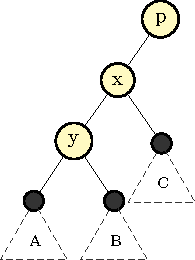
\includegraphics[width=\linewidth, page=1]{tree-rb-rightRotation}
		\caption{Stato iniziale}
	\end{subfigure}\hfill
	\begin{subfigure}[t]{.23\linewidth}
		\includegraphics[width=\linewidth, page=2]{tree-rb-rightRotation}
		\caption{Il sottoalbero \(B\) diventa figlio sx di \(x\)}
	\end{subfigure}\hfill
	\begin{subfigure}[t]{.23\linewidth}
		\includegraphics[width=\linewidth, page=3]{tree-rb-rightRotation}
		\caption{\(x\) diventa figlio dx di \(y\)}
	\end{subfigure}\hfill
	\begin{subfigure}[t]{.23\linewidth}
		\includegraphics[width=\linewidth, page=4]{tree-rb-rightRotation}
		\caption{\(y\) diventa figlio di \(p\),\\il vecchio padre di \(x\)}
	\end{subfigure}
	\caption{Esempio di rotazione a destra}
\end{figure}

\clearpage
\subsection*{Inserimento di un nodo in un albero binario bilanciato}

Per inserire un nodo in un albero Red-Black si usa la stessa procedura usata per gli alberi binari di ricerca e si colora il nuovo nodo di \RED.
Il vincolo che potremmo violare è il terzo, quello che prevede che entrambi i figli di un nodo rosso siano neri.

\begin{algorithm}[H]
	\caption{Inserimento di un nodo in un \textsc{Red-Black Tree}}
	%&../preamble

% arara: pdflatex: { synctex: no }
% arara: latexmk: { clean: partial }
\ifstandalone
\begin{document}
\begin{algorithm}[H]
\fi

\BlankLine
\tcp{Inserimento di un nodo in un albero Red-Black}
\prototype{\Tree \insertNode{\Tree T, \Tree k, \Item x}}{
	\Tree \(p \Assign \Nil\) \Comment*[l]{riferimento al padre}
	\Tree \(u \Assign T\) \Comment*[l]{riferimento alla radice}

	\BlankLine
	\tcp{cerco posizione inserimento}
	\While{\(u \Neq \Nil\) \And \(u.\treeKey \Neq k\)}{
		\(p \Assign u\)\;
		\(u\) \Assign \iif{\(k < u.\treeKey, u.\treeLeft, u.\treeRight\)}\;
	}

	\BlankLine
	\eIf{\(u \Neq \Nil\) \And \(u.\treeKey \Equal k\)}{
		\tcp{la chiave è già presente, aggiorno il valore}

		\BlankLine
		\(u.\treeValue \Assign v\)\;
	}{
		\tcp{la chiave non è presente}
		\tcp{creo un nodo coppia chiave-valore}
		\Tree \(new\) \Assign \treeConstructor{\(k, v\)}\;

		\BlankLine
		\tcp{collego il nodo creato}
		\shortcut{\(p, new, k\)}\;

		\alert{\treeFixInsert{\(new\)}}\;

		\BlankLine
		\If{\(p \Equal \Nil\)}{
			\(T \Assign new\) \Comment*[l]{primo nodo ad essere inserito}
		}
	}

	\BlankLine
	\tcp{restituisco l'albero non modificato o il nuovo nodo}
	\Return \(T\)\;
}

\ifstandalone
\end{algorithm}
\end{document}
\fi

\end{algorithm}

Nel caso in cui l'inserimento vìoli il terzo vincolo ci sposteremo verso l'alto lungo il percorso di inserimento;
cercheremo di ripristinare il terzo vincolo;
sposteremo le violazioni verso l'alto rispettando il quarto vincolo (mantenendo l'altezza nera dell'albero);
al termine, coloreremo la radice di nero (onorando il primo vincolo).

\begin{note}
Le operazioni di ripristino sono necessarie solo quando due nodi consecutivi sono rossi, altrimenti non sono necessarie.
\end{note}

\clearpage
\begin{algorithm}[H]
	\caption{Bilanciamento dell'albero in seguito all'inserimento di un nodo rosso}
	\setcounter{AlgoLine}{0}
	%&../preamble

% arara: pdflatex: { synctex: no }
% arara: latexmk: { clean: partial }
\ifstandalone
\begin{document}
\begin{algorithm}[H]
\fi

\BlankLine
% \tcp{bilanciamento di un \textsc{Red-Black Tree} in seguito all'inserimento di un nodo \RED}
\prototype{\treeFixInsert{\Tree t}}{

	\BlankLine
	\(t.\treeColor \Assign \RED\) \Comment*[l]{coloro il nodo da inserire di rosso}

	\BlankLine
	\tcp{\(t \Equal \Nil\) è la condizione di fino ciclo}
	\While{\(t \Neq \Nil\)}{

		\BlankLine
		\lnlset{case:refences}{0}%
		\Tree \(p \Assign t.\treeParent\) \Comment*[r]{riferimento al padre}
		\Tree \(n \Assign\) \iif{\(p \Neq \Nil, p.\treeParent, \Nil\)} \Comment*[r]{riferimento al nonno}
		\Tree \(z \Assign\) \iif{\(n \Equal \Nil, \Nil\), \iif{\(n.\treeLeft \Equal p, n.\treeRight, n.\treeLeft\)}} \Comment*[r]{riferimento allo zio}

		\BlankLine
		\lnl{case:no-father}%
		\uIf{\(p \Equal \Nil\)}{
			\(t.\treeColor \Assign \BLACK\)\;
			\(t \Assign \Nil\) \Comment*[l]{fine}
			\BlankLine

		}%
		\lnl{case:black-father}
		\uElseIf{\(p.\treeColor \Equal \BLACK\)}{
			\(t \Assign \Nil\) \Comment*[l]{fine}
			\BlankLine

		}%
		\lnl{case:red-aunt}
		\uElseIf{\(z.\treeColor \Equal \RED\)}{
			\(p.\treeColor \Assign z.\treeColor \Assign \BLACK\)\;
			\(n.\treeColor \Assign \RED\)\;
			\(t \Assign n\) \Comment*[l]{passo il problema al nonno}
			\BlankLine

		}\Else{

			\BlankLine
			\lnlset{right-left}{4a}%
			\uIf{(\(t \Equal p.\treeRight\)) \And (\(p \Equal n.\treeLeft\))}{
				\leftRotation{\(p\)}\;
				\(t \Assign p\) \Comment*[l]{passo il problema al padre}
				\BlankLine

			}%
			\lnlset{left-right}{4b}%%
			\eIf{(\(t \Equal p.\treeLeft\)) \And (\(p \Equal n.\treeRight\))}{
				\rightRotation{\(p\)}\;
				\(t \Assign p\) \Comment*[l]{passo il problema al padre}
				\BlankLine

			}{%
				\BlankLine
				\lnlset{left-left}{5a}%
				\uIf{(\(t \Equal p.\treeLeft\)) \And (\(p \Equal n.\treeLeft\))}{
					\rightRotation{\(n\)}\;
				}%
				\lnlset{right-right}{5b}%
				\ElseIf{(\(t \Equal p.\treeRight\)) \And (\(p \Equal n.\treeRight\))}{
					\leftRotation{\(n\)}\;
				}

				\BlankLine
				\(p.\treeColor \Assign \BLACK\)\;
				\(n.\treeColor \Assign \RED\)\;
				\(t \Assign \Nil\) \Comment*[l]{fine}
			}
		}
	}
}

\ifstandalone
\end{algorithm}
\end{document}
\fi

\end{algorithm}

\clearpage
\begin{enumerate}[label={\footnotesize\ttfamily (\arabic*)}, start=0]

	\vspace{-5pt}
	\item dichiaro dei riferimento al padre, al nonno e allo zio
	\begin{figure}[H]\centering
		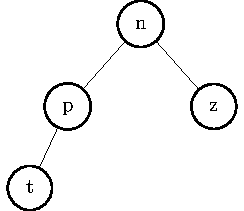
\includegraphics[page=1]{tree-rb-insertNode}
	\end{figure}

	\vspace{-5pt}
	\item il nuovo nodo \(t\) non ha padre; Questo può accadere in due casi:
		\begin{compactlist}
			\item è il primo nodo ad essere inserito, oppure
			\item quando abbiamo spostato la violazione verso l'alto fino a raggiungere la radice
		\end{compactlist}
	Ricoloriamo \(t\) di \BLACK in quanto trovandosi sulla radice dell'albero non viola nessun vincolo.

	\vspace{-5pt}
	\begin{figure}[H]\centering
		\begin{subfigure}[t]{.5\textwidth}\centering
			\includegraphics[width=.3\linewidth, page=2]{tree-rb-insertNode}
			\caption{Possibile violazione del primo vincolo}
		\end{subfigure}%
		\begin{subfigure}[t]{.5\textwidth}\centering
			\includegraphics[width=.3\linewidth, page=3]{tree-rb-insertNode}
			\caption{Ricolorazione del nodo \(t\)}
		\end{subfigure}
		% \caption{Spostamento del problema verso l'alto}
	\end{figure}

	\vspace{-5pt}
	\item il padre \(p\) di \(t\) è nero; anche in questo caso non abbiamo violato nessun vincolo perché avendo inserito un nodo rosso la lunghezza dei cammini neri non cambia e avendo inserito un nodo rosso figlio di un nodo nero non violiamo il terzo vincolo;

	\vspace{-5pt}
	\begin{figure}[H]\centering
		\includegraphics[page=4]{tree-rb-insertNode}
	\end{figure}

	\vspace{-5pt}
	\item il padre \(p\) e lo zio \(z\) sono rossi; Se \(z\) è rosso è possibile ricolorare di nero \(p\) e \(z\), e di rosso \(n\); poiché tutti i cammini che passano per \(z\) e \(p\) passano anche per \(n\), l'altezza nera non è cambiata (non abbiamo violato il quarto vincolo); Abbiamo spostato così il problema verso l'alto, più precisamente sul nonno che potrebbe aver violato il primo o il terzo vincolo, ovvero che \(n\) può essere una radice rossa o che abbia un padre rosso. Per risolvere il problema poniamo \(t \Assign n\) e continuiamo il ciclo.

	\vspace{-5pt}
	\begin{figure}[H]\centering
		\begin{subfigure}[t]{.5\textwidth}
			\includegraphics[width=\linewidth, page=5]{tree-rb-insertNode}
			\caption{Possibile violazione del primo e del terzo vincolo}
		\end{subfigure}%
		\begin{subfigure}[t]{.5\textwidth}
			\includegraphics[width=\linewidth, page=6]{tree-rb-insertNode}
			\caption{Ricolorazione del padre e dello zio di nero}
		\end{subfigure}
		% \caption{Spostamento del problema verso l'alto}
	\end{figure}

	\item[\footnotesize\ttfamily (4a)] il padre \(p\) è rosso e lo zio \(z\) è nero; si assuma che \(t\) sia figlio \emph{destro}  di \(p\) e che \(p\) sia figlio \emph{sinistro}  di \(n\); effettuando una rotazione a sinistra a partire dal nodo \(p\) scambiamo i ruoli di \(t\) e d \(p\) ottenendo il caso {\footnotesize\ttfamily (5a)}, dove i nodi in conflitto sul terzo vincolo sono entrambi figli \emph{sinistri} dei loro padri; i nodi coinvolti nel cambiamento sono \(p\) e \(t\), entrambi rossi, quindi l'altezza nera non cambia; abbiamo spostato il problema al padre, quindi poniamo \(t \Assign p\) e continuiamo il ciclo.

	\item[\footnotesize\ttfamily (4b)] speculare al caso {\footnotesize\ttfamily (4a)} (ossia che che \(t\) sia figlio \emph{sinistro}  di \(p\) e che \(p\) sia figlio \emph{destro}  di \(n\))

	\begin{figure}[H]\centering
		\begin{subfigure}[t]{.5\textwidth}
			\includegraphics[width=\linewidth, page=7]{tree-rb-insertNode}
			\caption{Possibile violazione del primo e del terzo vincolo}
		\end{subfigure}%
		\begin{subfigure}[t]{.5\textwidth}
			\includegraphics[width=\linewidth, page=8]{tree-rb-insertNode}
			\caption{Ricolorazione del padre e dello zio di nero}
		\end{subfigure}
		\caption[]{Rappresentazione grafica del caso {\footnotesize\ttfamily (4a)}}
	\end{figure}

	\item[\footnotesize\ttfamily (5a)] anche in questo caso il padre \(p\) è rosso e lo zio \(z\) è nero; ma si assuma che \(t\) sia figlio \emph{sinistro} di \(p\) e che \(p\) sia figlio \emph{sinistro}  di \(n\); effettuando una rotazione a destra a partire dal nodo \(n\) ci porta ad una situazione in cui \(t\) e \(n\) sono figli di \(p\); colorando \(p\) di nero ed \(n\) di rosso ci troviamo in una situazione in cui tutti i vincoli vengono rispettati (in particolare, l'altezza nera che passano per la radice è uguale a quella iniziale).

	\item[\footnotesize\ttfamily (5b)] speculare al caso {\footnotesize\ttfamily (5a)} (ossia che che che \(t\) sia figlio \emph{destro} di \(p\) e che \(p\) sia figlio \emph{destro}  di \(n\))

	\begin{figure}[H]\centering
		\begin{subfigure}[t]{.5\textwidth}
			\includegraphics[width=\linewidth, page=8]{tree-rb-insertNode}
			\caption{Possibile violazione del primo e del terzo vincolo}
		\end{subfigure}%
		\begin{subfigure}[t]{.5\textwidth}
			\includegraphics[width=\linewidth, page=9]{tree-rb-insertNode}
			\caption{Ricolorazione del padre e dello zio di nero}
		\end{subfigure}
		\caption[]{Rappresentazione grafica del caso {\footnotesize\ttfamily (5a)}}
	\end{figure}
\end{enumerate}

\paragraph{Complessità}
Ognuna di queste operazione avviene in tempo costante.
Ogni volta il problema può salire di uno o due livelli, in quanto l'altezza dell'albero è limitata da \(\log n\), il nostro algoritmo è limitato superiormente da \(\log n\), ossia \(\Omicron(\log n)\).

Più precisamente:
\begin{itemize}
	\item \(\Omicron(\log n)\) per scendere fino al punto di inserimento;
	\item \(\Omicron(1)\) per effettuare l'inserimento;
	\item \(\Omicron(\log n)\) per risalire ed \enquote{aggiustare} (caso {\footnotesize\ttfamily 3})
\end{itemize}

\clearpage
\subsection*{Esempi di inserimento}

Proviamo ad inserire il nodo \(16\) nell'albero red-black sottostante.

\begin{figure}[H]\centering
	% \renewcommand{\subfigurename}{Es.}
	% \renewcommand\thesubfigure{\arabic{subfigure}}
	% \captionsetup[subfigure]{labelformat=simple, labelsep=space}
	\begin{subfigure}[t]{.48\linewidth}\centering
		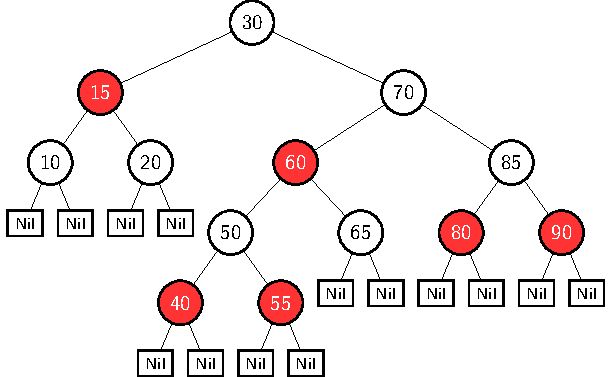
\includegraphics[width=\linewidth, page=1]{tree-rb-insertNode-example-1}
		\caption{Stato attuale}
	\end{subfigure}
	\hfill
	\begin{subfigure}[t]{.48\linewidth}\centering
		\includegraphics[width=\linewidth, page=2]{tree-rb-insertNode-example-1}
		\caption{Inserimento del nodo \(16\) andato a buon fine}
	\end{subfigure}
\end{figure}

\vspace{-5pt}
Non violiamo alcun vincolo in quanto il padre di \(16\) è nero e non abbiamo modificato l'altezza nera.
Questo caso rappresenta il caso {\footnotesize\ttfamily 2}, l'inserimento del nodo \(16\) è quindi andato a buon fine.
Alternativamente proviamo ad inserire il nodo \(42\) sempre nello stesso albero.

% \vspace{-5pt}
\begin{figure}[H]\centering
	\begin{subfigure}[t]{.48\linewidth}\centering
		\includegraphics[width=\linewidth, page=2]{tree-rb-insertNode-example-2}
		\caption{Inserimento del nodo \(42\), violiamo il secondo vincolo, ci troviamo nel caso {\footnotesize\ttfamily 3} (\(z\) rosso), quindi coloriamo di nero \(p\) e \(z\) e di rosso \(n\), il problema si sposta ad \(n\)}
	\end{subfigure}
	\hfill
	\begin{subfigure}[t]{.48\linewidth}\centering
		\includegraphics[width=\linewidth, page=3]{tree-rb-insertNode-example-2}
		\caption{Violiamo il terzo vincolo, entrambi i nodi rossi sono figli \emph{sinistri} quindi ci troviamo nel caso {\footnotesize\ttfamily 5a}, quindi coloriamo di nero \(p\), di rosso \(n\) \dots}
	\end{subfigure}

	\vspace{5pt}

	\begin{subfigure}[t]{.48\linewidth}\centering
		\includegraphics[width=\linewidth, page=4]{tree-rb-insertNode-example-2}
		\caption{\dots ed effettuiamo una rotazione a destra con perno \(n\)}
	\end{subfigure}
	\hfill
	\begin{subfigure}[b]{.48\linewidth}\centering
		\includegraphics[width=\linewidth, page=5]{tree-rb-insertNode-example-2}
		\caption{Abbiamo ripristinato il terzo vincolo, gli altri vincoli non sono mai stati violati, quindi abbiamo finito}
	\end{subfigure}
\end{figure}
\vspace{-10pt}

Questo esempio ci mostra chiaramente come gli alberi Red-Black, attraverso il rispetto dei vincoli, tendano a mantenere bilanciato l'albero.
Esiste una versione \emph{top-down} dell'algoritmo di inserimento che scende fino interessato \enquote{aggiustando} l'albero man mano.

\clearpage
\subsection{Rimozione di un nodo}

Se il nodo rimosso è rosso l'altezza nera rimane invariata, non sono stati creati nodi rossi consecutivi e la radice resta nera.
Il problema sorge quando si rimuovono nodi neri in quanto è possibile che siano stati violati il primo ed il terzo vincolo e sicuramente è stato violato il quarto vincolo in quanto cambia l'altezza nera.
L'algoritmo \treeFixDelete{\(T, t\)} ripristina la proprietà Red-Black con rotazioni e cambiamenti di colore.
Ci sono quattro casi possibili (e 4 simmetrici).
% A lezione non è stato spiegato l'algoritmo, viene riportato solo per completezza.

\vspace{-5pt}
\begin{algorithm}[H]
	\caption{Rimozione di un nodo in un \textsc{Red-Black Tree}}
	% \caption{Bilanciamento dell'albero in seguito alla rimozione di un nodo}
	% NOTE non presente nel documento finale
	% \input{tree-rb-removeNode}
	\setcounter{AlgoLine}{0}
	%&../preamble

% arara: pdflatex: { synctex: no }
% arara: latexmk: { clean: partial }
\ifstandalone
\begin{document}
\begin{algorithm}[H]
\fi

\BlankLine
% \tcp{bilanciamento di un \textsc{Red-Black Tree} in seguito alla rimozione di un nodo \RED}
\prototype{\treeFixDelete{\Tree T, \Tree t}}{

	\BlankLine
	\(t.\treeColor \Assign \RED\) \Comment*[l]{coloro il nodo da inserire di rosso}

	\BlankLine
	\While{(\(t \Neq T\)) \And (\(t.\treeColor \Equal \BLACK\))}{

		\BlankLine
		\Tree \(p \Assign t.\treeParent\) \Comment*[r]{riferimento al padre}

		\BlankLine
		\eIf{\(t \Equal p.\treeLeft\)}{

			\BlankLine
			\Tree \(f \Assign p.\treeRight\) \Comment*[r]{riferimento al fratello}
			\Tree \(ns \Assign f.\treeLeft\) \Comment*[r]{riferimento al nipote sinistro}
			\Tree \(nd \Assign f.\treeRight\) \Comment*[r]{riferimento al nipote destro}

			\BlankLine
			\lnl{caso1}%
			\eIf{\(f.\treeColor \Equal \RED\)}{
				\(p.\treeColor \Assign \RED\)\;
				\(f.\treeColor \Assign \BLACK\)\;
				\leftRotation{\(p\)}\;
				\tcp{t viene lasciato inalterato, quindi si ricade nei casi 2, 3, 4}
				\BlankLine

			}{

				\lnl{caso2}%
				\uIf{\(ns.\treeColor \Equal nd.\treeColor \Equal \BLACK\)}{
					\(f.\treeColor \Equal \RED\)\;
					\(t \Assign p\) \Comment*[l]{passo il problema al padre}
					\BlankLine

				}%
				\lnl{caso3}%
				\uElseIf{(\(ns.\treeColor \Equal \RED\)) \And (\(nd.\treeColor \Equal \BLACK\))}{
					\(ns.\treeColor \Assign \BLACK\)\;
					\(f.\treeColor \Assign  \RED\)\;
					\rightRotation{\(f\)}\;
					\tcp{t viene lasciato inalterato, quindi si ricade nel caso 4}
					\BlankLine

				}%
				\lnl{caso4}%
				\ElseIf{\(nd.\treeColor \Equal \RED\)}{
					\(f.\treeColor \Equal p.\treeColor\)\;
					\(p.\treeColor \Assign \BLACK\)\;
					\(nd.\treeColor \Assign \BLACK\)\;
					\leftRotation{\(p\)}\;
					\(t \Assign T\)\;
				}
			}
		}{
			\tcp{casi speculari}
		}
	}
}

\ifstandalone
\end{algorithm}
\end{document}
\fi

\end{algorithm}
\vspace{-10pt}

La cancellazione è concettualmente complicata, ma è efficiente.
\begin{enumerate}[label={\footnotesize\ttfamily (\arabic*)}, noitemsep, topsep = 5pt, parsep = 5pt, partopsep = 0pt]
	\item si passa ad uno dei casi 2, 3, 4;
	\item si torna ad uno degli altri casi, ma risalendo di un livello l'albero;
	\item si passa al caso 4;
	\item si termina.
\end{enumerate}

% \paragraph{Complessità}
\`{E} possibile visitare al massimo un numero \(\Omicron(\log n)\) di casi, ognuno dei quali è gestito in \(\Omicron(1)\).

\ifsubfile
\end{document}
\fi
